%\documentclass[10pt,a4paper]{article}
\documentclass[12pt,a4paper]{article}
\usepackage{graphicx,units,amsmath}
\usepackage{bm} % bold in math mode
\usepackage{subfigure}
\usepackage{float}
\usepackage[ngerman, english]{babel} 
%\usepackage[utf8]{inputenc}
\setcounter{secnumdepth}{4}

\usepackage[top=2cm, bottom=2.5cm, left=3cm, right=3cm]{geometry}

%-Eingabe der Metadaten des Titelblattes--------------------------

%-Daten des Autors / Authors Data---------------------------------

\newcommand{\dcauthorpre}{~} 
\newcommand{\dcauthorsurname}{Kullmann} 
\newcommand{\dcauthorname}{Richard} 
\newcommand{\dcauthoradd}{geboren am 17.07.1996 in Berlin-Pankow}

%-Titel und Untertitel / Title and subtitle-----------------------

\newcommand{\dctitle}{Giant Diffusion in two-dimensional Neuron Models} 
\newcommand{\dcsubtitle}{~}  
% Falls dcsubtitle NICHT verwendet werden soll, {\dcsubtitle}{~} eingeben.

%-Eingabe der Betreuuernahmen / Names of the consultants---------

\newcommand{\dcconsulta}{~} 
\newcommand{\dcconsultb}{~} 
\newcommand{\dcconsultc}{~} 

%-Eingabe der Gutachternamen / Names of the approvals-------------

\newcommand{\dcapprovala}{Prof. Dr. Benjamin Lindner} 
\newcommand{\dcapprovalb}{Prof. Dr. Igor Sokolov} 
\newcommand{\dcapprovalc}{~} 

%-Information zur Universitaet------------------------------------

\newcommand{\dcdegree}{Master of Science\\(M. Sc.)} 
\newcommand{\dcsubject}{Physik} 
\newcommand{\dcfaculty}{Mathematisch-Naturwissenschaftlichen Fakult\"at I}
\newcommand{\dcinstitute}{Institut f\"ur Physik}
\newcommand{\dcuniversity}{Humboldt-Universit\"at zu Berlin}
\newcommand{\dcdean}{Prof. Dr. sc. Heinz  M\"uller}
\newcommand{\dcpresident}{Prof. Dr. Dr. h.c. Wilhelm Schulz}

%-Pruefungsdaten: eingereicht und mdl. Pruefung-------------------
%-data of submission and oral exam--------------------------------

\newcommand{\dcdatesubmitted}{5. Juni 2020} %auch wenn nicht auf dem 
%Titelblatt, bitte erf�llen!
\newcommand{\dcdateexam}{2. Juli 1999} 


% Folgende Zeile bitte nicht aendern!
\newcommand{\dckeywordsde}{\vfill \raggedright {\textbf{Schlagw\"orter:}}\\ \dckeydea, \dckeydeb, \dckeydec, \dckeyded \\}

%-englische Schlagwoerter / english keywords----------------------

\newcommand{\dckeyena}{Giant Diffusion}
\newcommand{\dckeyenb}{Two-Dimensional Neuron Models}
\newcommand{\dckeyenc}{Bistability}
\newcommand{\dckeyend}{Signal-to-Noise Ratio}

% Folgende Zeile bitte nicht aendern!
\newcommand{\dckeywordsen}{\vfill \raggedright {\textbf{Keywords:}}\\ \dckeyena, \dckeyenb, \dckeyenc, \dckeyend \\}

\newcommand{\dcpdfsubject}{Dissertation}  
\graphicspath{{images/}}
\begin{document}


%\title{Masterarbeit}
%\author{Richard Kullmann}
%\date{15.07.2019}

%----------Generierung der Titelseite-----bitte nicht ver�ndern!--------------------


\author{von \\ \dcauthorpre\ \dcauthorname\ \dcauthorsurname\ \\ \dcauthoradd}

%----------
\title{ \vspace{-2cm}\dctitle \\ 
\vspace{0.5cm}
\large{\dcsubtitle} \\ 
\vspace{0.5cm} {\Large{MASTERARBEIT}}\\ 
\vspace{0.5cm} \large{zur Erlangung des akademischen Grades \\ 
\dcdegree\\ im Fach \dcsubject \\\vspace{0.5cm}

\includegraphics[width=6cm]{husiegel}\\ 
\vspace{0.5cm} eingereicht an der \\ 
\dcfaculty \\ 
\dcinstitute\\
\dcuniversity \\}}
%-----------------
\date{\vspace{2.5cm}
%\raggedright{
%Pr\"asident der Humboldt-Universit\"at zu Berlin:\\
%\dcpresident \vspace{-0.3cm}
%}\vspace{0.5cm}\\
%
%\raggedright{
%Dekan der \dcfaculty:\\
%\dcdean \vspace{-0.3cm}
%}\vspace{0.5cm}\\
%
% auskommentiert weil nicht standard
\raggedright{
Gutachter:
\begin{enumerate} 
\item{\it\dcapprovala} \vspace{-0.3cm}
\item{\it\dcapprovalb} \vspace{-0.3cm}
%\item{\it\dcapprovalc} \vspace{-0.3cm}
\end{enumerate}} \vspace{0.5cm}
%\raggedright{
%Betreuung:
%\begin{enumerate} 
%\item{\it\dcconsulta} \vspace{-0.2cm}
%\item{\it\dcconsultb} \vspace{-0.2cm}
%\end{enumerate}} \vspace{0.5cm}
%-----------------
\raggedright{
\begin{tabular}{lll}
eingereicht am: &  &\it\dcdatesubmitted\\ % wenn nicht in der Pr�fungsordnung, die Zeile bitte auskommentieren
%Tag der m\"undlichen Pr\"ufung: & & \dcdateexam
\end{tabular}}\\ 
}
%------------------------------------- 

\maketitle

\thispagestyle{empty}
%\setcounter{page}{2}
\newpage
%-englische-Zusammenfassung---------------------------------------

%\selectlanguage{english}

%\begin{abstract}
%\setcounter{page}{2} % Nach Bedarf anpassen!
%Here is the english abstract.\\
% hier werden die englische Schlagw�rter aus Metadaten �bernommen
%\dckeywordsen				
%\end{abstract}

%-deutsche Zusammenfassung----------------------------------------

%\selectlanguage{german}

\begin{abstract}
\setcounter{page}{2} % Nach Bedarf anpassen!
The emerging field of magnetometry based on NV centers opens a variety of new experimental perspectives, including the imaging of single nuclear spins on the nanoscale. However, in order to achieve exceptionally long NV electron spin coherence times and high sensitivities, the NV spin needs to be decoupled from unwanted interactions with the environment. This can be accomplished with dynamical decoupling sequences.
\\
During the work for this thesis, multiple dynamical decoupling protocols were implemented and tested on NV centers in bulk diamond and nanodiamond. 
\\
The theoretical part covers general NV properties before treating the behaviour of a free electron spin and finally applying this on the NV center. Then, the effect of different decoupling protocols are discussed. After that, the structure and concept of the setup will be explained. In the final part, the measurements will be presented. The execution of the decoupling sequences will be demonstrated and the data will be used to extract the spectral density function of the environment.
\\
It was shown that all implemented dynamical decoupling sequences could enhance the coherence time. It was demonstrated that CPMG outperforms the other sequences on the given setup, achieving an improvement of up to a factor of 200 in the bulk diamond and 50 in nanodiamond. Finally, the examination of the spectral density functions of the spin bath gave a deeper insight in its coupling strength to the NV and its internal dynamics.\\
In the future, the limitations of the sequences will be further explored and other decoupling protocols will be tested. In addition to that, a better time and phase control has to be accomplished. These efforts will eventually lead to sensitivities high enough to detect small spin ensembles and even single molecular spins.
% hier werden die deutsche Schlagw�rter aus Metadaten �bernommen
%\dckeywordsde
\end{abstract}
\thispagestyle{empty}

\tableofcontents
\thispagestyle{empty}
\newpage
\pagenumbering{arabic}

\section{Introduction}

The human brain is one of the most investigated but still least understood subjects in scientific research. This comes as no surprise considering the huge variety of tasks it can perform efficiently and seemingly effortlessly: it constantly combines multiple sensory impressions and filters the most relevant of them to form a coherent image of the surroundings, it remembers information it has learned decades ago, it can produce the most complex thoughts and keep a whole organism working properly in the meantime. And despite the mayor improvement of processor performance and increasing interest in machine learning and artificial neural networks during the past couple of years, no technological implementation has even remotely managed to match the capability of the human brain.\\
The basis for its high functionality lies in the huge number of neurons - around 100 Billions\cite{eqnum} - and their interconnectivity: neural cells usually receive inputs from more than 10.000 other neurons\cite{izi}. Thus, in order to be able to understand how the brain works and possibly derive future applications from that, it is crucial to examine neural cells and study their characteristics. \\
Neural cells display a plethora of responses to their synaptic inputs. In general, neural activity can be divided into four mayor regimes: resting state, sub-threshold oscillations, spiking and bursting\cite{dnb}. This work will focus on bursting neurons. These exhibit phases of repetitive spiking followed by periods of quiescence. A comparable behaviour was observed for Brownian Particles underlying bistable velocity dynamics\cite{abp}\cite{bpp}, induced either via a velocity potential or movement in a biased cosine potential. In these systems, a specific range of parameters leads to diverging diffusion coefficients for vanishing noise intensity. This phenomenon is called \glqq Giant Diffusion \grqq. Applying this observation to neural cells, this could mean a large enhancement of the Signal-to-Noise Ratio through just a slight change in the system parameters. The goal of this thesis is to find out whether Giant Diffusion can be observed in a simple two-dimensional neuron model and which consequences this might have on the signal transmission, e.g. the Signal-to-Noise Ratio when the system is subject to an external stimulus.

\section{Theory}
\subsection{Quantities of interest}
In the context of Brownian Motion, there are two characteristic quantities: the ensemble of particles moves with a mean velocity
\begin{equation}
\left\langle v\right\rangle =\lim_{t\rightarrow\infty}\frac{\left\langle x(t)-x(0) \right\rangle}{t}
\end{equation}
and is subject to a diffusive spread around this average flow that can be described by the effective diffusion coefficient
\begin{equation}
D_{eff}=\lim_{t\rightarrow\infty}\frac{\left\langle x^2(t) \right\rangle-\left\langle x(t)\right\rangle ^2}{2t}
\end{equation}
For the investigation of neuron models, a third quantity needs to be considered, namely the Fano factor:
\begin{align*}
F=\frac{\left\langle \Delta N^2(t) \right\rangle}{\left\langle N(t)\right\rangle}
\end{align*}
In order to compare the neuron model with Brownian Particles, one may also define a Fano factor for mechanical systems:
\begin{align*}
F=\frac{2D_{eff}}{L\langle v\rangle}
\end{align*}
where $L$ can be chosen arbitrarily, e.g. a characteristic length of the system, so that $F$ becomes dimensionless.
\subsection{Giant Diffusion}
The term \glqq Giant Diffusion \grqq is short for \textit{Giant Enhancement of (thermal) diffusion} which was first observed around the turn of the millennium for Brownian Particles in a tilted periodic potential\cite{td}\cite{ga}\cite{dit}\cite{gd}. In general, these particles exhibit two stable velocity states. They can be \glqq trapped\grqq in a potential minimum - this is referred to as the \textit{locked state} - or they can be in the \textit{running state}. A particle gets into the running state if it has managed to overcome a hill and the frictional loss is low enough so that it is able to pass the adjacent hills as well. In the case of large friction or a strongly tilted potential, however, only one of these two states is present. If the potential is tilted in such a way that both states exist and the probabilities to be in either state are similar, many switchings between the states will occur. In the weak-noise-limit, half of the particles will be mainly in the locked state, while for the others the running state prevails. This behavior leads to diverging diffusion coefficients known as Giant Diffusion.
\subsection{Giant diffusion of Brownian Particles}
First observed by the botanist Robert Brown in 1828\cite{bm}, the term \textit{Brownian Motion} describes the irregular movement of particles in a viscous medium, whose apparently random changes of direction are caused by collisions with smaller particles or molecules.
\\
Ordinary Brownian Motion obeys a simple linear Langevin-equation:
\begin{align*}
\text{m}\dot{v}=-\lambda v+\xi(t)
\end{align*}
The evolution of the velocity $v$ of the particle is affected by a linear friction term with coefficient $\lambda$ and a random force $\xi(t)$. \\
\\ 
In the following, two different systems with Brownian Motion dynamics exhibiting Giant Diffusion are presented. These were the motivation for my research on bursting neuron models.
\subsubsection{Active Brownian Particles}
Active Brownian Motion can be observed on small organisms, like bacteria or cells, which are able to move on their own. In order to model the behaviour of such an object, a more general friction term needs to be introduced into the Langevin-equation:
\begin{align*}
\dot{v}=-f(v)+\xi(t)
\end{align*}
Here, the noise was assumed to be additive and the mass was omitted due to clarity.
An accurate description of the self-propulsion can be accomplished by choosing the function $f$ in such a way that it attains negative values at small velocities and becomes greater than zero at large speed. Thus, at small velocities the particle will accelerate and with increasing velocity, regular friction will start to affect its motion.
\\
A system like this was studied by Lindner and Nicola in 2008\cite{abp}. They chose a cubic function for the friction term, $f(v)=v-v^3+F$, allowing them to write the equation of motion in terms of a quartic velocity potential $U(v)$:
\begin{equation}
\dot{v}=-U'(v)+\xi(t)
\end{equation}
with $U(v)=\frac{1}{4}v^4-\frac{1}{2}v^2-Fv$.
\begin{figure}[H]
	\centering
	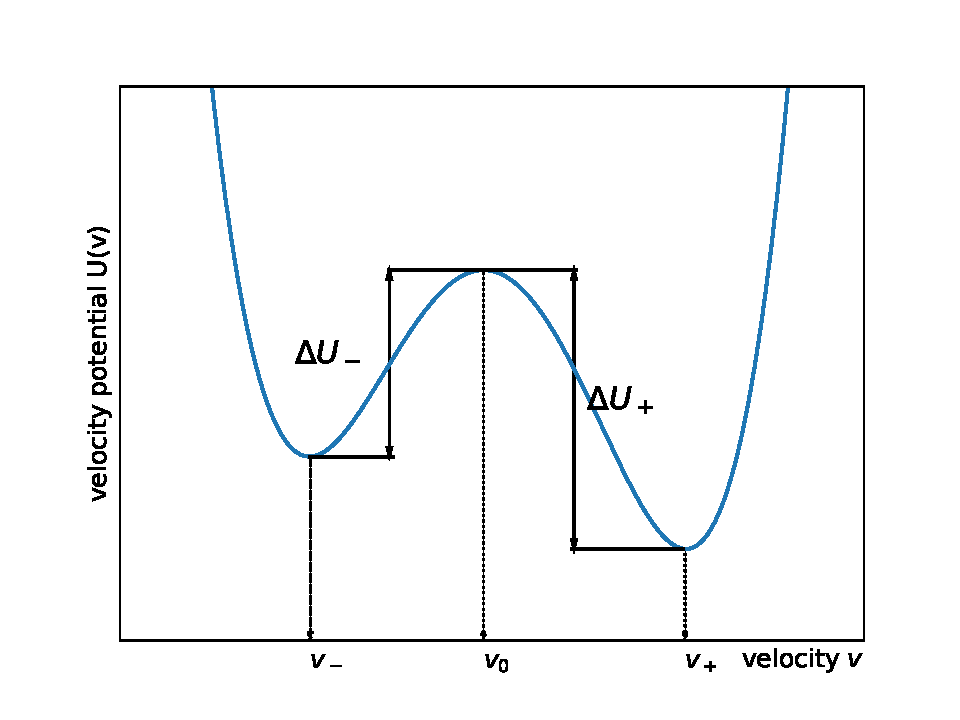
\includegraphics[scale=1]{velpot.pdf} 
	\caption{tilted velocity potential of an Active Brownian Particle}
	\label{velpot}
\end{figure}
This potential shows two minima at $v_\pm$, representing the stable velocity states \glqq forwards\grqq and \glqq backwards\grqq, and a maximum at $v_0$. In order to transition from $v_\pm$ into the other state, the particle needs to overcome a barrier of height $\Delta U\pm$.  
\\
Their simulations revealed a certain region of bias forces $F$, in which giant diffusion occurred.
\begin{figure}[H]
	\centering
	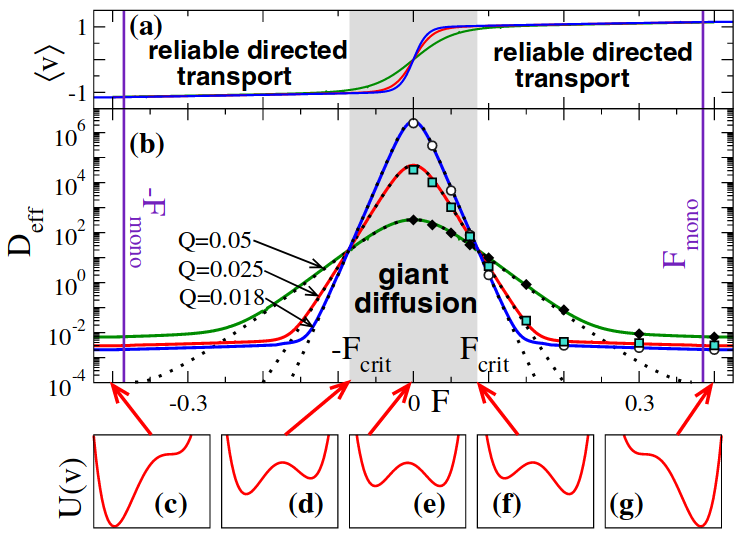
\includegraphics[scale=0.5]{mess08.png}\caption{Simulation of velocity and effective diffusion coefficient for Active Brownian Particles underlying a tilted velocity potential,taken from \cite{abp}}
	\label{abpsim}
\end{figure}
Inside this region, the diffusion coefficients increase with decreasing noise intensity, while they decrease outside of this region. In other words, in the weak noise limit, the diffusion coefficients diverge in the critical region and vanish outside of it. The critical force lies at the border of this region and emerges from the intersection points of the diffusion coefficients for different noise levels. A simple criterion could be found for these intersection points: at the critical force, one potential barrier is twice as high as the other potential barrier. 
Furthermore, it is remarkable that the reliable directed transport which takes place outside of the critical region appears much earlier than the monostability of the velocity potential, which is a obviously only a primitive criterion for reliable transport in one direction. 
The mean velocity displays a more regular behavior. It is almost constant at a value less than zero up to small negative forces, then undergoes a sharp increase to a positive value and barely changes afterwards. They intersect as well, approximately at the position where the diffusion coefficient gets maximal.
\subsubsection{Regular Brownian Particles in a tilted periodic potential}
On their own, ordinary Brownian Particles do not exhibit bistable velocity dynamics which may lead to giant diffusion. But as mentioned before, this can be done by adding a periodic potential to the equation of motion:
\begin{equation}
\dot{v}=-\gamma v-U'(x)+\sqrt{2\gamma kT}\xi(t)
\end{equation}
with $U(x)=-Fx-d\cos(x)$. This system was discussed with respect to giant diffusion in a paper by Lindner and Sokolov from 2016\cite{bpp}. Now, in contrast to the Active Brownian Particle, the evolution of the system is not governed by a velocity potential, but by a spatial potential:
\begin{figure}[H]
	\subfigure[]{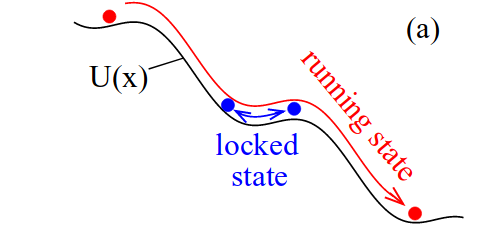
\includegraphics[width=0.5\textwidth]{veldynupper.png}} 
	\subfigure[]{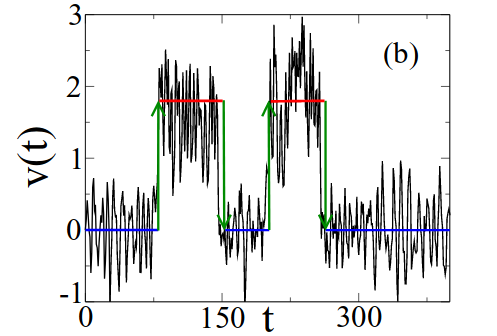
\includegraphics[width=0.5\textwidth]{veldynlower.png}} 
	\caption{Figure (a) visualizes the motion of a Brownian Particle in a periodic potential, on the right one can see the bistable velocity dynamics. The oscillations thereby arise from local extrema of the potential.}
	\label{veldyn} 
\end{figure}
Also for the Brownian Particles in a cosine potential, there was a finite range of bias forces, for which giant diffusion could be observed:
\begin{figure}[H]
	\centering
	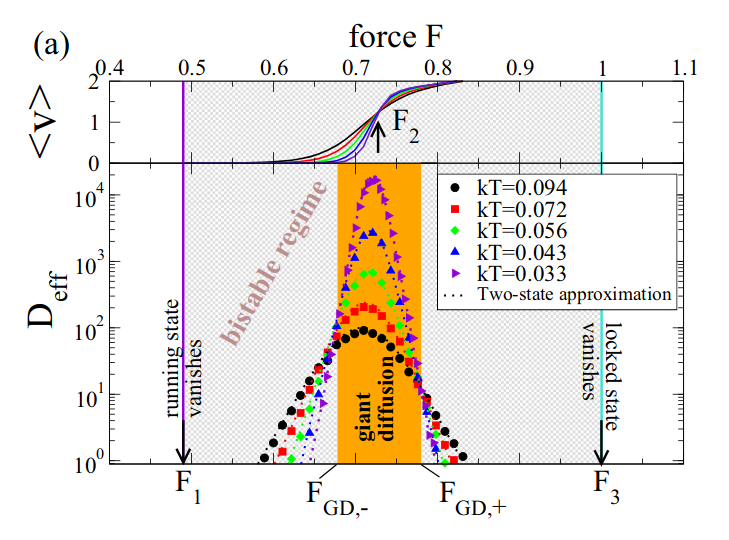
\includegraphics[scale=0.5]{nbpsim1.png}\caption{Simulation of velocity and effective diffusion coefficient for Brownian Particles in a tilted periodic potential,taken from \cite{bpp}}
	\label{anbpsim}
\end{figure}
Again, all curves of the diffusion coefficient intersect at two points and diverge in between those points for decreasing noise intensities while going to zero on the outside and the velocity curves intersect approximately at the maximum of the diffusion coefficient. And also here the region of giant diffusion is much smaller than the range of bias forces, where both states coexist. Two other variables that help characterize the system are the transition rates between the states, that is from the locked to the running state and vice versa. Even though there didn't exist actual potential barriers, these turned out to obey an Arrhenius or Kramers law, respectively, as can be seen from an Arrhenius plot:
\begin{figure}[H]
	\centering
	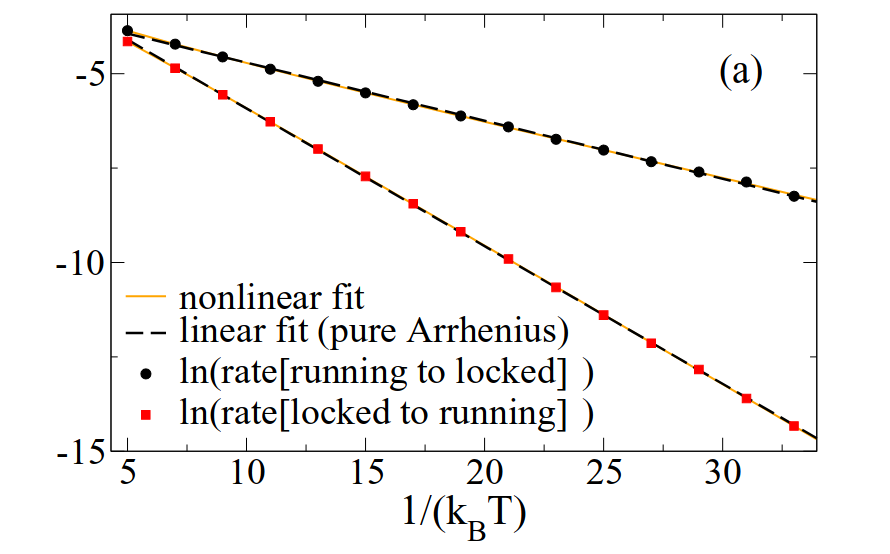
\includegraphics[scale=0.5]{kramerfit.png}\caption{Fits of the transition rates with both an Arrhenius and a Kramers law, taken from \cite{bpp}}
	\label{bparr}
\end{figure}
In this example, the Arrhenius fit as well as the Kramers fit yield good agreements with the data. From these fits one can extract effective potential barriers. The relation found for the potential barriers of the Active Brownian Particle can be tested by plotting the effective barriers and twice their value:
\begin{figure}[H]	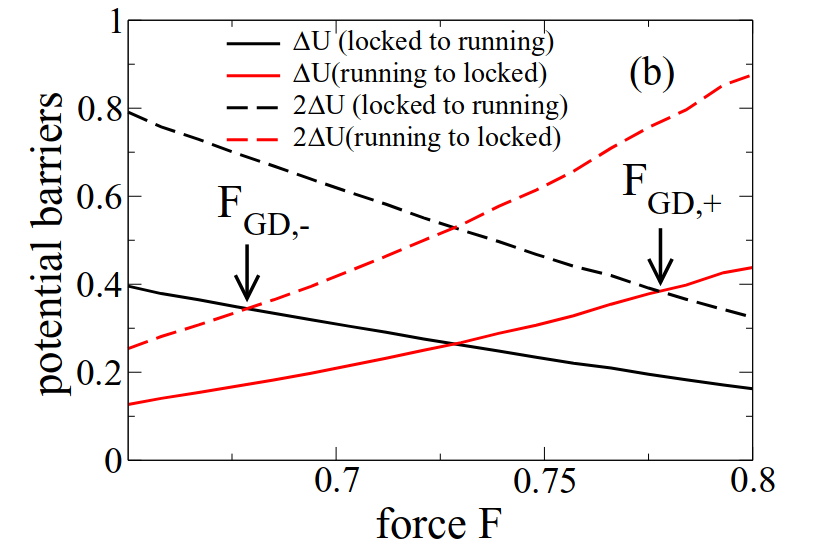
\includegraphics[scale=0.5]{barrierplot.png}\caption{Plot of the effective potential barriers. The dotted curves are simply twice the solid curves of the same color. This plot is taken from \cite{bpp}}
\end{figure}
The plot shows that the points where one potential barrier equals twice the other roughly correspond to the critical forces, so the criterion applies as well to this case, where no potential barriers were present and only effective barriers could be calculated.
\subsection{Two-state theory}\label{tst}
In the case of low noise intensity, the transition times between the locked state and the running state will be much shorter than the periods of time that the particle stays in one of the two states. That is why it is practical to describe the behavior of the system in this regime with a two-state model. The following derivation applies to the Brownian Particle in a tilted periodic potential. The transition rates are assumed to obey an Arrhenius law:
\begin{align*}
r_{\pm}=r_{0,\pm}\exp\left(-\frac{\Delta U_{\pm}}{D}\right)
\end{align*}
where $r_-$ denotes the transition rate from locked to running state, and $r_+$ the rate for the other transition. $\Delta U_{\pm}$ is the corresponding potential barrier and $D$ the noise intensity. The effective diffusion coefficient can be calculated from the velocity $v_0$ in the running state and the transition rates: 
\begin{align*}
D_{\text{eff}}=\frac{v_0^2 r_+r_-}{(r_++r_-)^3}
\end{align*}
The first task is to find the intersection points of the diffusion coefficients. At these points, the diffusion coefficients become independent of the noise intensity.
It is
\begin{align*}
D_{\text{eff}}&=\frac{v_0^2r_{0,+}r_{0,-}\exp\left(-\frac{\Delta U_++\Delta U_-}{D}\right)}{\left[r_{0,+}\exp(\frac{-\Delta U_+}{D})+r_{0,-}\exp\left(\frac{-\Delta U_-}{D}\right)\right]^3}\\&=\frac{v_0^2r_{0,+}r_{0,-}}{\left[r_{0,+}\exp\left(-\frac{3\Delta U_+-\Delta U_+-\Delta U_-}{3D}\right)+r_{0,-}\exp\left(-\frac{3\Delta U_--\Delta U_+ -\Delta U_-}{3D}\right)\right]^3}\\&=\frac{v_0^2r_{0,+}r_{0,-}}{\left[r_{0,+}\exp\left(-\frac{2\Delta U_+-\Delta U_-}{3D}\right)+r_{0,-}\exp\left(-\frac{2\Delta U_--\Delta U_+}{3D}\right)\right]^3}
\end{align*}
In the limes $D\rightarrow 0,\Delta U_+>U_-$ the first term in the denominator vanishes, resulting in:
\begin{align*}
D_{\text{eff}}=\frac{v_0^2r_{0,+}}{r_{0,-}^2}\exp\left(-\frac{\Delta U_+-2\Delta U_-}{D}\right)
\end{align*}
Under the assumption that the prefactors change slowly in comparison to the exponential function, the following condition arises:
\begin{align*}
\Delta U_+=2\Delta U_-
\end{align*}
Due to symmetry of the problem, the opposing case $D\rightarrow 0,\Delta U_+<U_-$ yields:
\begin{align*}
\Delta U_-=2\Delta U_+
\end{align*}
In both cases, one potential barrier is twice as high as the other one.\\
Next, we will examine whether the Fano factor displays similar features in the weak noise limit. As 
\begin{align*}
F=\frac{2D_{\text{eff}}}{L\langle v\rangle}
\end{align*}
an expression for the average velocity is required to compute the Fano factor. Taking into account that the average velocity is zero when the particle is in the locked state, one finds the following formula for the total mean velocity:
\begin{align*}
\langle v\rangle=v_0\frac{r_-}{r_++r_-}
\end{align*}
Therefore
\begin{align*}
F=\frac{2v_0r_+}{(r_++r_-)^2}=\frac{2v_0r_{0,+}\exp\left(\frac{-\Delta U_+}{D}\right)}{\left(r_{0,+}\exp\left(\frac{-\Delta U_+}{D}\right)+r_{0,-}\exp\left(-\frac{\Delta U_-}{D}\right)\right)^2}
\end{align*}
In the limes $D\ll1$ there are again two solutions. For $\Delta U_+ > \Delta U_-$:
\begin{align*}
F=\frac{2v_0r_{0,+}}{r_{0,-}^2}\exp\left(-\frac{\Delta U_+-2\Delta U_-}{D}\right) \rightarrow \Delta U_+=2\Delta U_-
\end{align*}
as well as for $\Delta U_+ < \Delta U_-$:
\begin{align*}
F=\frac{2v_0}{r_{0,+}}\exp\left(-\frac{\Delta U_+-2\Delta U_+}{D}\right) \rightarrow \Delta U_+=0
\end{align*}
The intersection point for $\Delta U_+ > \Delta U_-$ stays the same while at the other critical point the potential barrier from running to locked state needs to vanish. As the latter condition violates the requirements for the application of the two-state theory - because only one state would exist in this case - the second intersection point can't be determined via this two-state model.
\section{Giant diffusion in a bursting neuron model}
\subsection{Brownian motion and neuronal models}
Brownian motion in periodic potentials has numerous applications among which one can find superionic conduction, rotation of a dipole in a static field or the description of a Josephson Tunneling junction\cite{fpe}. However, apart from these mechanical examples, Brownian motion in periodic potentials is also suited to describe a bursting neuron. If one counts every time the particle crosses a hill as a spike, the running state can be associated with tonic firing and the locked state with a stable equilibrium point. Because of the random noise, transition between the states will occur and the sustained spiking will be eventually terminated so that there is only a finite number of spikes within each burst. The position of the Brownian Particle then corresponds to the spike count of the neuron and its velocity to the firing rate. Thus, based on the similarities to Brownian motion, we expect to find a weak noise behavior comparable to giant diffusion also in bursting neurons.
\subsection{Neuronal bursting}
Depending on its physiology and the properties of the stimulus, a neuron doesn't always fire a single spike. A series of multiple spikes in a short time interval that is followed by a period of quiescence is called a burst\cite{izi}. Typically, bursting results from the interplay between two subsystems: a fast subsystem, that is responsible for the generation of the spikes within a burst, and a slow subsystem that modulates the bursting pattern and eventually terminates sustained spiking. However, a bursting neuron model that implements these slow and fast dynamics would at least have to be three-dimensional, as there would be a variable for the membrane voltage as well as for the fast and slow oscillations. One way to realize a bursting two-dimensional model and to make use of the various methods of phase plane analysis is to introduce noise into the system. Considering that any neuron is subject to some kind of noise, this is a justified assumption and was even proposed by Izhikevich as a way to make two-dimensional neuronal models burst\cite{izi}.
\subsection{The bursting neuron model}
The main focus of this thesis lies on the study of the $I_{Na,p}+I_K$-model, the persistent sodium plus potassium model with additive noise:
\begin{align}\label{Veq}
C\dot{V} &= I - g_L(V-E_L) - g_{Na}m_{\infty}(V)(V-E_{Na}) - g_Kn(V-E_K)+\sqrt{2D}\xi(t)\\\label{neq}
\dot{n} &= (n_{\infty}(V)-n)/\tau(V)
\end{align}
Here, $V$ denotes the mambrane voltage, $C$ is the capacitance, $I$ is the bias current, $g_i$ are conductances and $E_i$ the Nernst equilibrium potentials. The overall noise intensity is $D$. Lastly, $m_{\infty}$ is the activation variable of the instantaneous $Na^+$ current, while $n$ governs the variation of the slower $K^+$ current. The steady-state activation functions are approximated by the Boltzmann-function:
\begin{align*}
f_{\infty}(V) = \frac{1}{1+\exp\{(V_{1/2}-V)/k\}}
\end{align*}
At $V_{1/2}$, the activation function has the value 1/2, and $k$ is the slope factor determining the steepness around $V_{1/2}$ - a smaller value of $k$ leads to a more abrupt change of $f_{\infty}$. This approximation was suggested by Izhikevich \cite{izi}.\\
The fastest neural oscillations in the human brain are gamma waves with frequencies in the range between 25 and 100 Hz\cite{gamma}\cite{gamma2}. Similar values can also be found in different papers about bursting neurons\cite{burstneu}\cite{burstneu2}. Therefore, the parameters were chosen such that the frequency in the bursting state was about 70 Hz.
The exact values used in the simulations were:\\\\
$C=1$ , $g_L=0.3$ , $E_L=-80$ , $g_{Na}=1$ , $E_{Na}=60$ , $g_K=0.4$ , $E_K=-90$.
\begin{align*}
\intertext{Instantaneous $Na^+$ current:} k_m&=14 , V_{1/2,m}=-18. 
\\
\intertext{$K^+$ current:} k_n&=5 , V_{1/2,n}=-25 , \tau(V)=\text{const}=3.
\end{align*}
\subsection{Phase plane analysis}
\subsubsection{Nullclines}
For a system that depends on the evolution of two state variables, in this case $V$ and $n$, some qualitative and quantitative analysis can be carried out in the phase plane. A neat way to obtain information about an unknown system is to calculate its nullclines. The nullclines are curves in the phase plane, where one of the state variables remains constant. Thus, the $V$-nullcline is defined by the condition $\dot{V}=0$ and the $n$-nullcline follows from $\dot{n}=0$. By crossing one of the nullclines, the system changes its direction with respect to the corresponding variable. As a consequence, each nullcline separates the phase space into two regions where one variable evolves in opposite directions. Taken together, the nullclines define four different regions of directions: one region each where both variables decrease or increase and two regions where one variable increases and the other decreases. Depending on the specific shape of the nullclines, these regions do not necessarily have to be coherent.\\
The $V$-nullcline can be obtained by setting the left side of equation (\ref{Veq}) to zero. In the $V$-$n$-plane, it can then be described by the function
\begin{align}
n(V)=\frac{I - g_L(V-E_L) - g_{Na}m_{\infty}(V)(V-E_{Na})}{g_K(V-E_K)}
\end{align} 
The $n$-nullcline is just
\begin{align}
n(V)=n_\infty(V)
\end{align}
The nullclines of the $I_{Na,p}+I_K$-model are shown in figure \ref{realnc}.\\
A second aspect of the nullclines are their intersection points. As both state variables remain constant when the nullclines intersect, these points are equilibrium points.\\
In general, there are three different types of equilibria: nodes, saddles and foci. These may be stable or unstable. Any trajectory in the phase space starting close enough to a stable equilibrium stays near it for all times. In contrast to that, an equilibrium is unstable, if at least one trajectory that starts arbitrarily close to it diverges from the equilibrium.
If they are in the vicinity of a node, all trajectories either converge to or diverge from it. In the case of a saddle, most trajectories first approach the equilibrium point and then diverge from it. Trajectories that start near a focus rotate around the equilibrium point and thereby get closer to or farther away from it. 
\subsubsection{Jacobian matrix of the system}
The equilibrium points can be characterized by studying the Jacobian matrix of the system at these points. A two-dimensional system can be written in the form
\begin{align}
\dot{x}=f(x,y)\\
\dot{y}=g(x,y)
\end{align}
Utilizing the fact that the functions $f$ and $g$ can be linearized near the equilibrium, which means they can be approximated by the first term of their Taylor expansion, one finds a linear system at the equilibrium $(x_0,y_0)$:
\begin{align}				
\left(\begin{matrix}\dot{u}\\\dot{w}
\end{matrix}\right)
=\left(\begin{matrix}a b\\
c d\end{matrix}\right)\left(\begin{matrix}u\\w\end{matrix}\right)=L\left(\begin{matrix}u\\w\end{matrix}\right)
\end{align}
where $u=x-x_0$, $w=y-y_0$, $L$ is the Jacobian matrix at equilibrium and the coefficients are the partial derivatives
\begin{align}
a=\frac{\partial f}{\partial x}(x_0,y_0),\qquad b=\frac{\partial f}{\partial y}(x_0,y_0) \\
c=\frac{\partial g}{\partial x}(x_0,y_0),\qquad d=\frac{\partial g}{\partial y}(x_0,y_0)
\end{align} 
Having determined the eigenvalues $\lambda_\pm$ and eigenvectors $ \boldsymbol{v_\pm}$ of $L$, a solution for the linear system can be constructed:
\begin{align}
\left(\begin{matrix}u(t)\\w(t)
\end{matrix}\right)=c_+\boldsymbol{v_+}\exp(\lambda_+t)+c_-\boldsymbol{v_-}\exp(\lambda_-t)
\end{align}
At this point, the connection between the Jacobian matrix and the different types of equilibria becomes clear. If both eigenvalues are real and have the same sign, both terms of the solution either grow or decay exponentially, meaning that the equilibrium is a node. If they are real with opposite signs, the equilibrium point is a saddle. Finally, if the eigenvalues are complex-conjugate, the solution oscillates, which makes the equilibrium a focus\cite{izi}.\\
When no bias current is applied (that is, I=0), the system features three equilibrium points:
\begin{figure}[H]
	\centering
	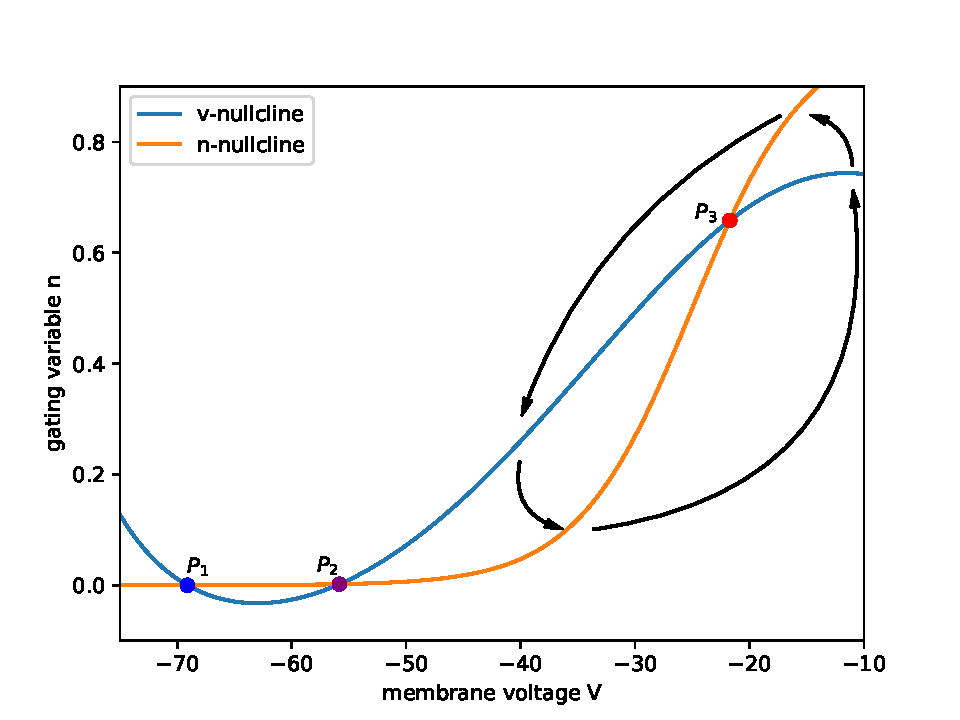
\includegraphics[scale=0.5]{inapikrealncwnp.pdf}\caption{Nullclines of the $I_{Na,p}+I_K$-model with $I=0$. The arrows indicate the direction of motion in the different regions.}
	\label{realnc}
\end{figure}
Carrying out the phase plane analysis, one finds:
\begin{align*}
\lambda_+(P_1)&\approx-0.1 & \lambda_-(P_1)&\approx-0.3\\
\lambda_+(P_2)&\approx 0.1& \lambda_-(P_2)&\approx -0.3\\
\lambda_+(P_3)&\approx 0.05 + 0.5i& \lambda_-(P_3)&\approx 0.05 - 0.5i
\end{align*}
This means that $P_1$ is a stable node, $P_2$ is a saddle point and $P_3$ is an unstable focus. Thus, in the bursting state, the phase vector will rotate around $P_3$, approach $P_2$ in $n$ - direction and then go away from $P_2$ in $V$ - direction in order to do another rotation around $P_3$.\\
However, this applies only to the case of small bias currents. When $I\approx 0.36$, the saddle and the node fall together and the system undergoes a saddle-node bifurcation. In this case, the resting state vanishes and the neuron is in a state of tonic spiking.
\subsection{Phenomenology}
The qualitative behavior of the neural model can be best understood by first considering the noiseless system. Depending on the choice of initial conditions, the system will start in either the resting or the running state and will not change its behavior anymore after a short period of equilibration, as can be seen in figure \ref{subfig}. 
\begin{figure}[H]
	\subfigure[]{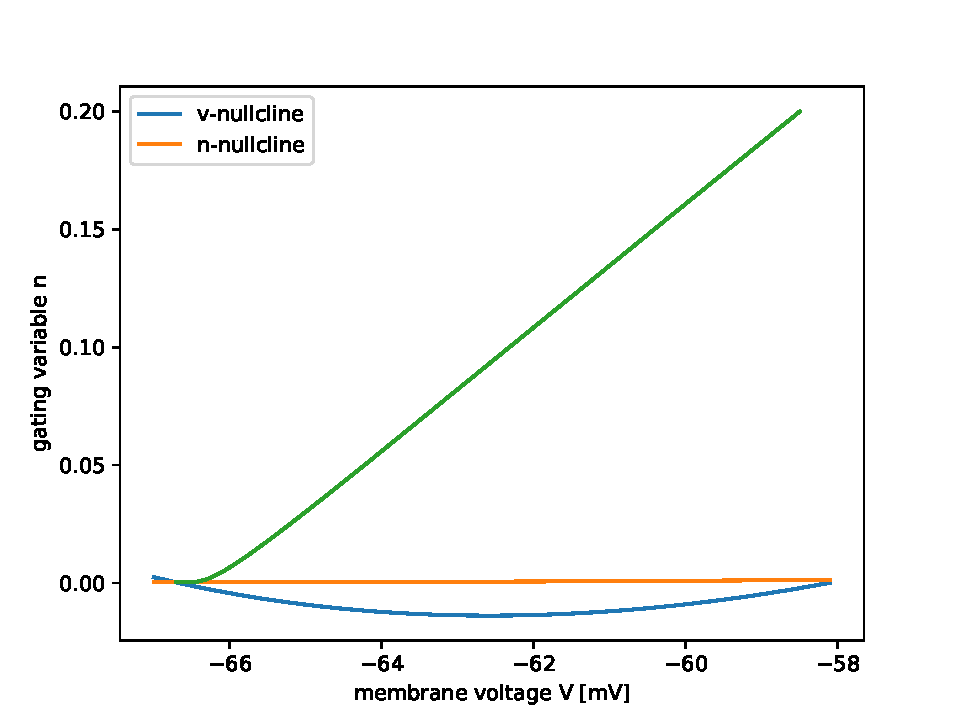
\includegraphics[scale=0.4]{inapreali20nbwn.pdf}} 
	\subfigure[]{	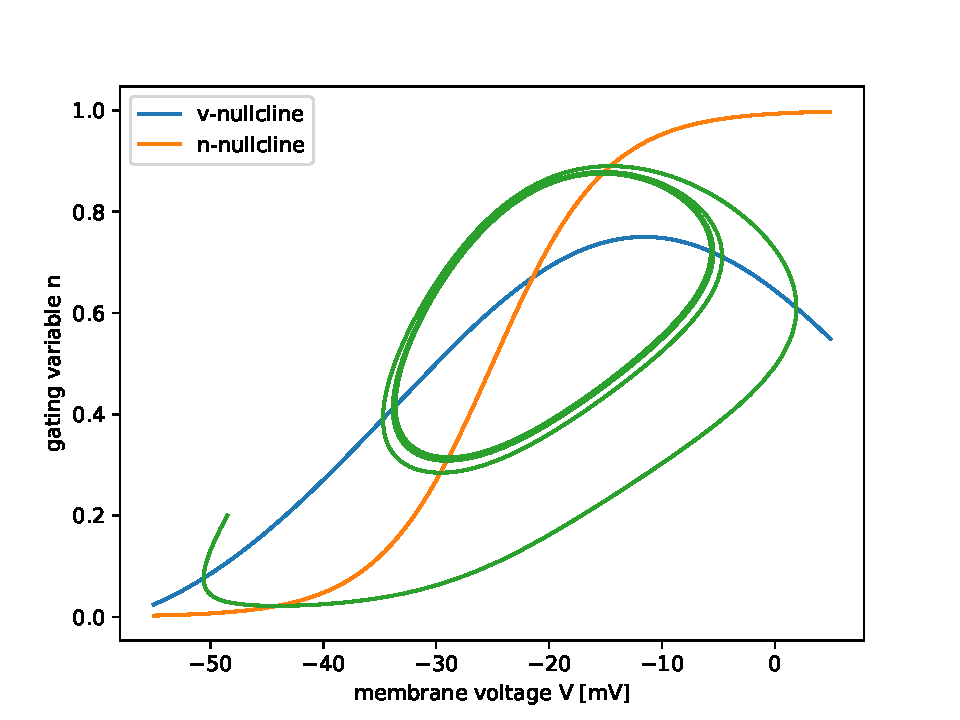
\includegraphics[scale=0.4]{inapreali20wn.pdf}}\\	\subfigure[]{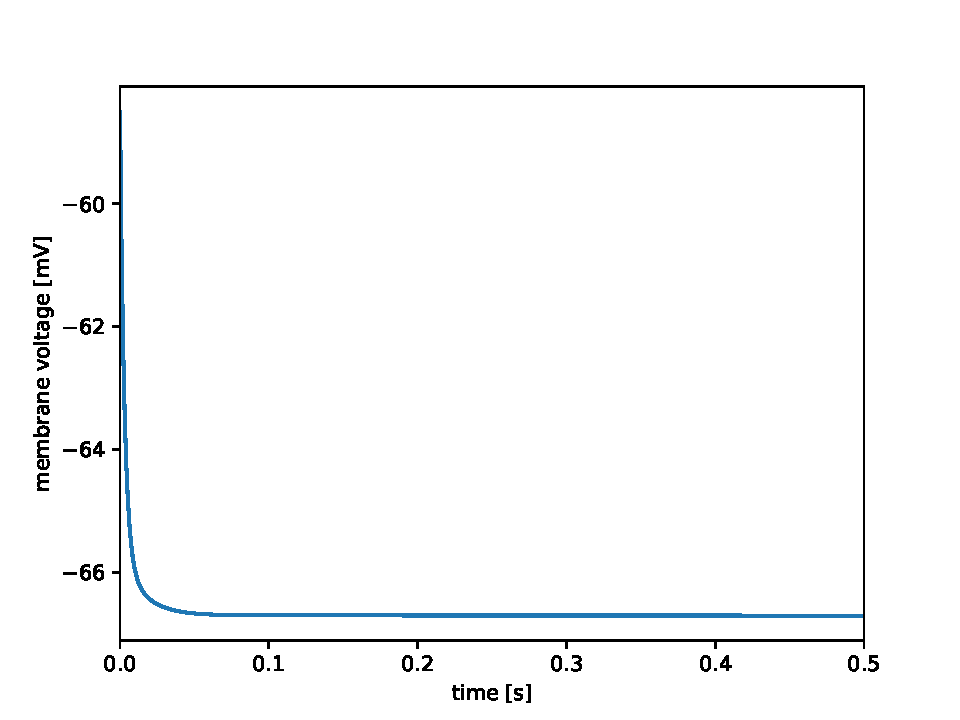
\includegraphics[scale=0.4]{inapreali20nbv.pdf}} 
	\subfigure[]{	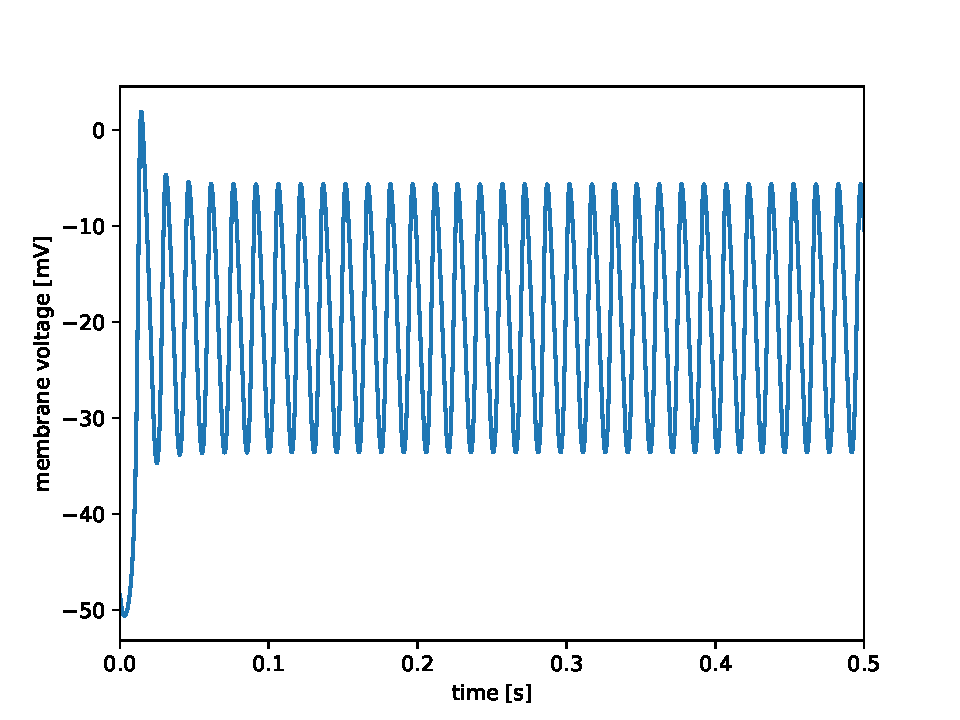
\includegraphics[scale=0.4]{inapreali20v.pdf}}
	\caption{Evolution of the phase vector (first row) and the membrane voltage over time (second row).
		The left side shows the evolution of the system with resting ICs, and on the right one can see the behavior under spiking ICs.}
	\label{subfig} 
\end{figure}
Analytically, it is hardly possible to determine whether a specific starting point ($V_0$,$n_0$) leads to repetitive spiking or no spiking at all. The only thing one can say for sure is that the line that separates both domains will go through the saddle point that was found in the phase plane analysis. Assuming that the gating variable does not change, any trajectory starting at higher voltages will lead to spiking while all trajectories at lower voltage converge to the stable node. A numerical investigation of the model without noise confirms our presumptions (figure \ref{twodom}).
\begin{figure}[H]
	\hspace*{-0.5cm}
	\subfigure[]{	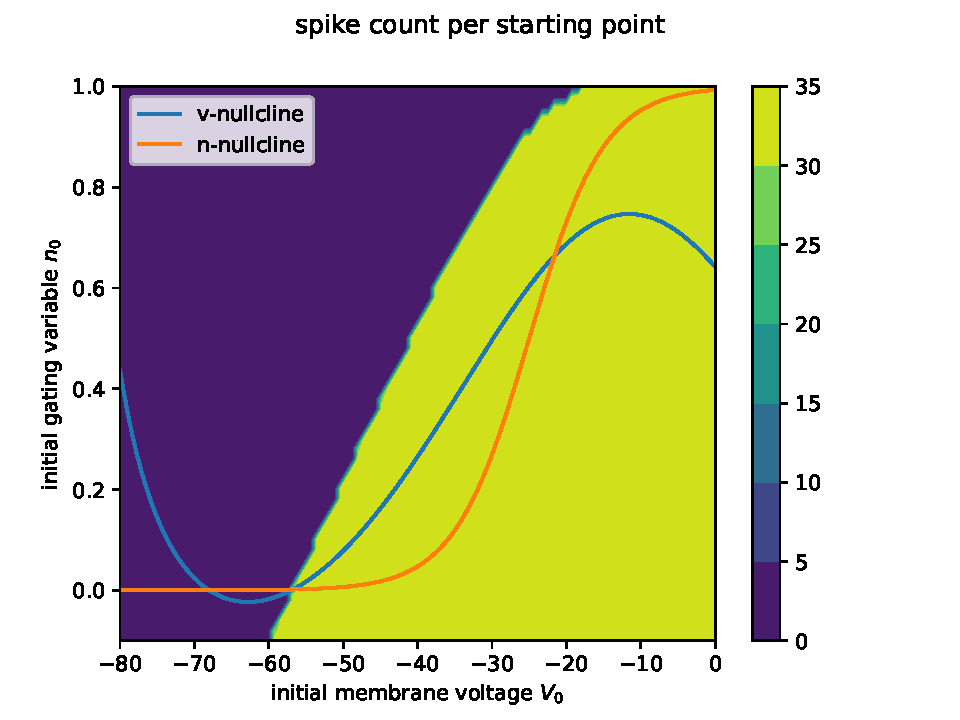
\includegraphics[scale=0.5]{contourneu01wnshort.pdf}}
	\subfigure[]{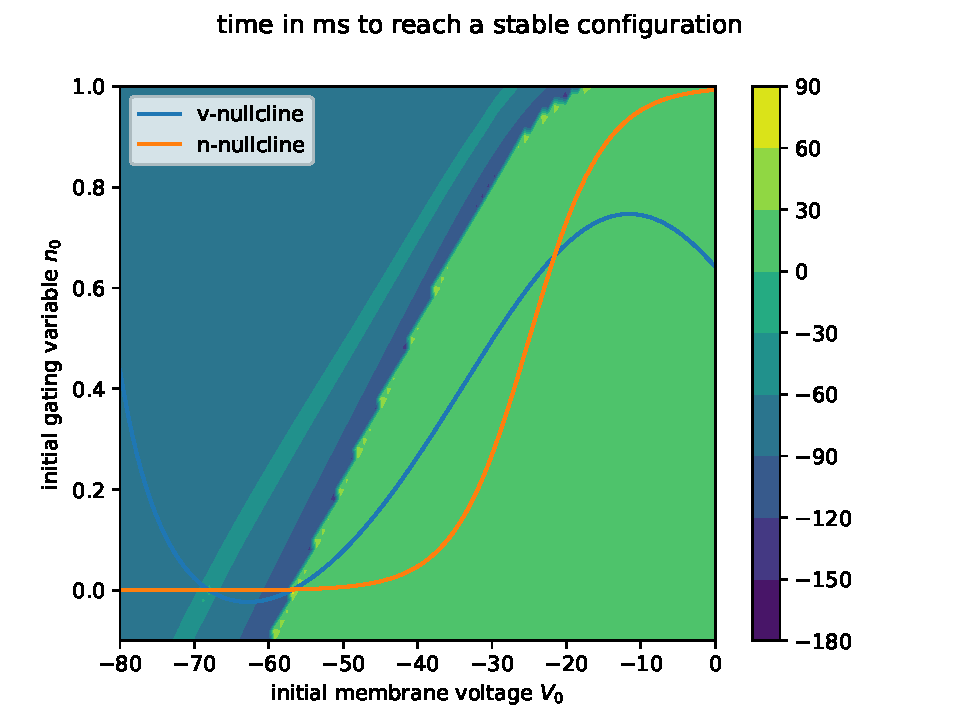
\includegraphics[scale=0.5]{contourtime01wn.pdf}}

	\caption{Phase plane image of the neuron model with $I=0.1$ and no noise. Each point represents a specific combination of starting parameters. The left plot shows the number of spikes over a short period of time and for the right picture, the equilibration times for both states were measured. The times to reach the stable node were multiplied with $-1$ so that a distinction between the states would be possible. Irregularities arise from the finite resolution of the $V_0$-$n_0$-lattice.}
	\label{twodom}
\end{figure}		
There are two distinct regions which can be separated by a monotonically increasing curve that passes through the saddle point. In figure \ref{twodom}b one can see a small intermediate area of large equilibration times. If the system parameters lie in the vicinity of this transition area, a small perturbation suffices to bring the system into either state. Remarkably, most of this area is made up by starting points leading to the stable equilibrium while only a small streak consists of bursting initial conditions. Consequently, the running state is reached much faster than the resting state.
\\
When noise is brought into the system, the findings for the noiseless system still apply to a great extent. Starting in one of the two domains, the system will most likely first converge to the corresponding state, and the time it takes for that will be about the same as before. However, the system will not stay in this state forever, but constantly perform noise-driven transitions between the states. Thus, it will not be possible anymore to assign an end state to each set of initial conditions. Obviously, both transition rates, meaning from running to resting and in the opposite direction, will grow when the noise intensity $D$ increases. \\
In addition to that, depending on the overall configuration, the system is usually biased towards one of the states. It is to be expected that at low bias current $I$, the resting state dominates and the running state is favored at high $I$. Considering the simulations (figure \ref{currentnoise}), this turns out to be a valid hypothesis: At $I=-0.1$, the neuron almost immediately returns to the resting state once it has gotten into the running state. At a slightly higher bias current of $I=0$, the periods of stay in both states are almost equal, and at $I=0.15$, the system is in the running state for the majority of time. The firing frequency in the running state lies at about 70 Hz.
\begin{figure}[H]
 	\subfigure[]{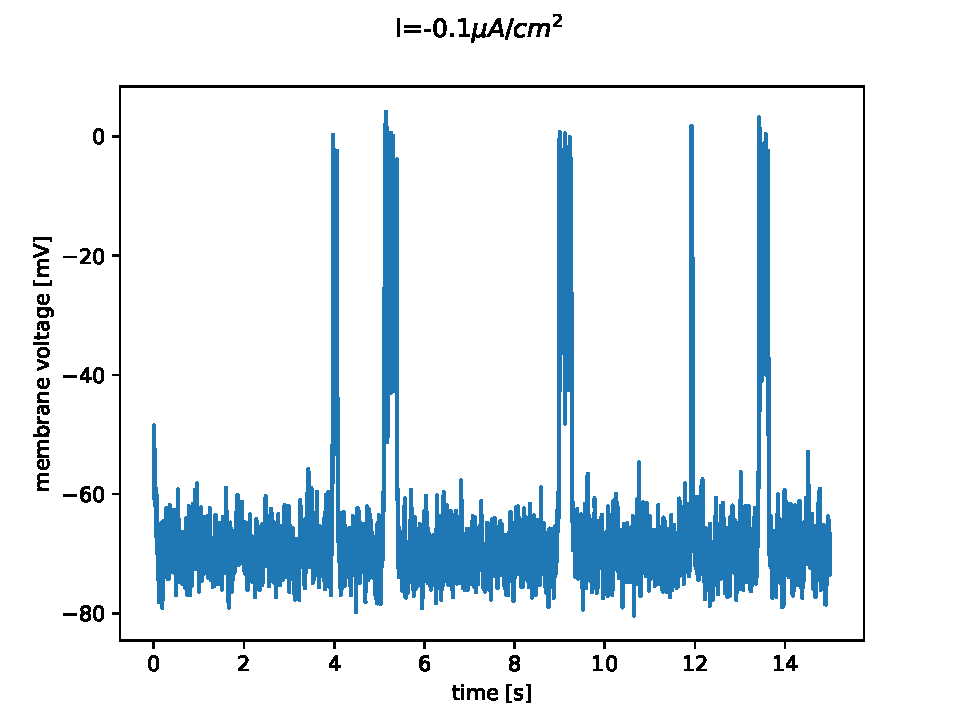
\includegraphics[scale=0.4]{realstate125.pdf}} 
 	\subfigure[]{	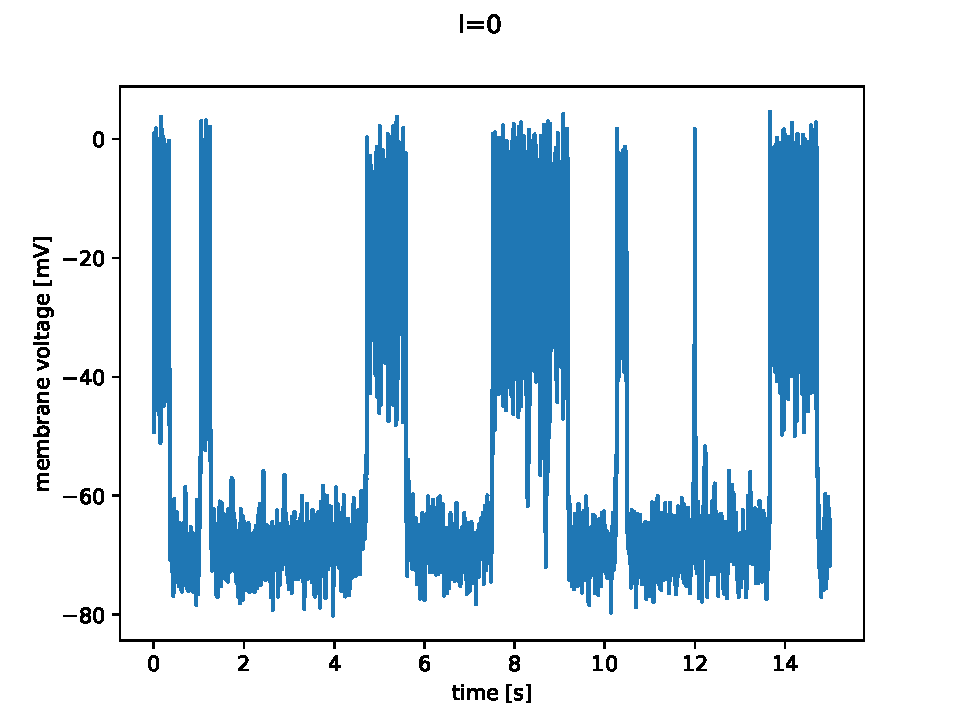
\includegraphics[scale=0.4]{realstate135.pdf}}\\	\subfigure[]{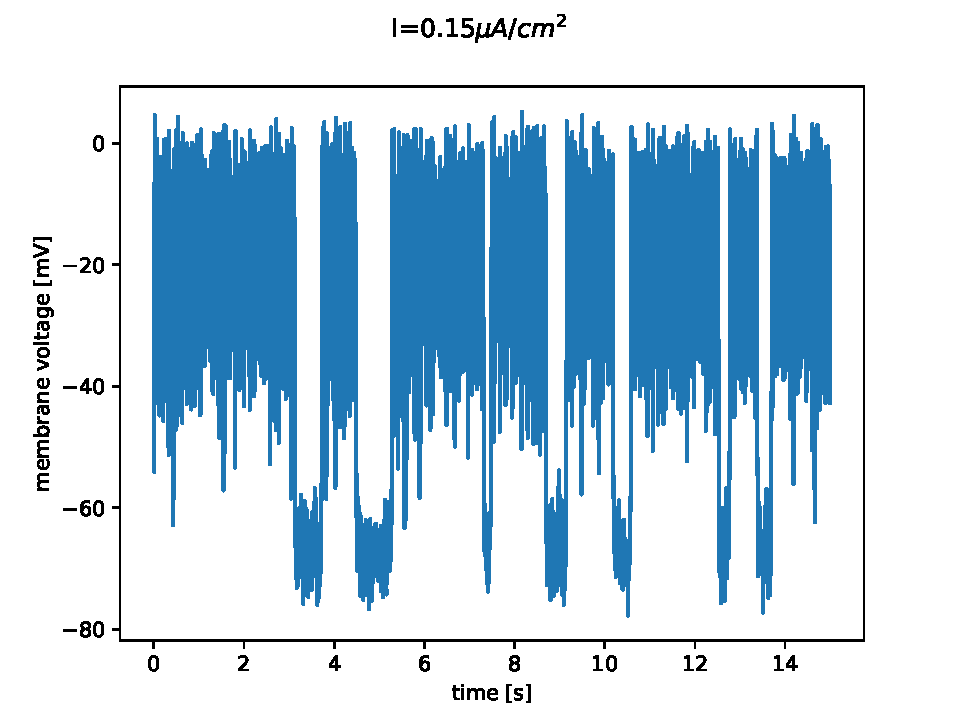
\includegraphics[scale=0.4]{realstate15.pdf}} 
 	\subfigure[]{	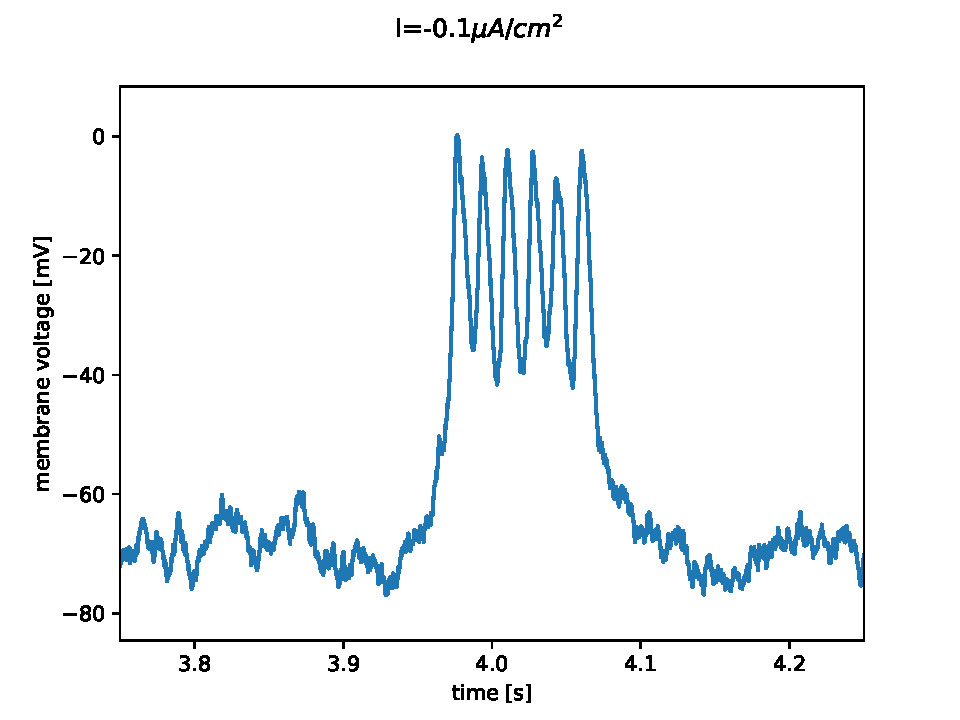
\includegraphics[scale=0.4]{realstate125vsh.pdf}}
 	\caption{Behavior of the membrane voltage for constant noise and changing bias current $I$. In figure (d), a segment with a higher time resolution is shown in order to better illustrate the evolution of the voltage variable.}
 	\label{currentnoise} 
 \end{figure}
In conclusion, the behavior of this two-dimensional bursting model displays the same characteristics as the Brownian particle in a tilted potential. Therefore, we expect to find similar count statistics and Giant Diffusion for this system as well. If this assumption is actually valid will be examined in the following chapter.

\section{Simulations}
\subsection{Numerics}
The behavior of the two-dimensional neuron model can be investigated by conducting simulations with the parameters described above and evaluating the data in a couple different ways. The simulations were done by letting the system evolve almost freely with the only external influence being the white gaussian noise with intensity $D$. \\
In all of the computations, only a single neuron was simulated over a long period of time. When investigating an ergodic system, this procedure ensures that the results are independent of the initial conditions if the simulation time is long enough. Furthermore, an ensemble of neurons would need to be equilibrated before starting any measurements so that the obtained results would be correct. This equilibration time can be omitted now, which saves some computation time. \\
Mostly, the spike train was cut into 500 segments. Only for $D=0.25$, the number of neurons was set to 50 so that there would be a higher number of transitions in a single voltage curve. In all cases, the timestep was 0.5 $\mu$s. The total measurement time for each spike train ranged from $5\cdot10^5$ s for high noise intensities to $2\cdot 10^6$ s for the lowest noise intensities, yielding lengths between $10^3$ and $4\cdot10^4$ for the segments.
\subsection{Count statistics}
The most characteristic feature of a neuron -from a mathematical point of view- is its spike count. Using the phase space description, the neuron produces a spike each time it performs a complete rotation around the instable equilibrium point or focus, respectively. This fact conveniently provides us with a numerical criterion for a spike:
every time the membrane voltage crosses the equilibrium value from below before the gating variable crosses its equilibrium value (also from below), a spike will be counted. \\
At $10^5$ different timepoints per segment, the spike count was combined with the spike counts from all the other segments in order to determine the effective diffusion coefficient $D_{eff}$, the fano factor $F$ and the average firing rate $r$. \\
The first quantity to be considered is $D_{eff}$.
As observed for the Brownian Particles, all curves intersect at two points which define the range of Giant Diffusion: between the intersection points, decreasing noise intensity leads to increasing diffusion and outside of the critical region, less noise leads to smaller diffusion. Thus, for $D=0.45$, the diffusion coefficient changes by approximately 3 orders of magnitude over the whole range of bias currents $I$ while the curve with $D=0.25$ already extends over 6 orders of magnitude. When halving the noise intensity roughly doubles the order of magnitudes in the measured diffusion coefficient, the effects of further reductions will be even greater. This makes it numerically very difficult to go beyond the values chosen in this plot.
\begin{figure}[H]
	\centering
	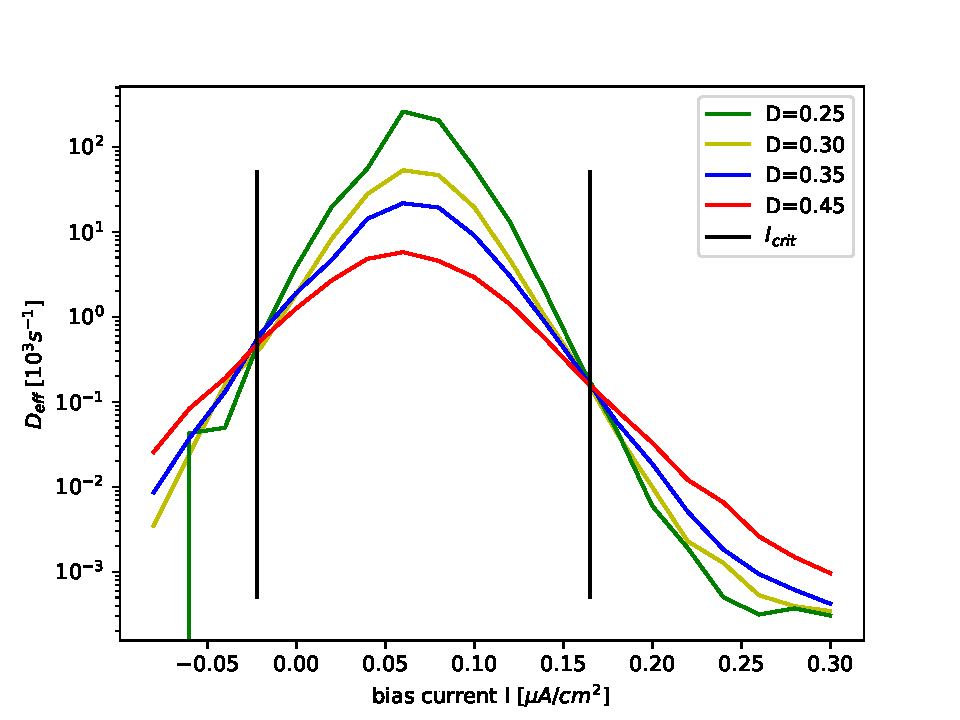
\includegraphics[scale=1]{deffcrit.pdf}\caption{Effective diffusion coefficients for different noise intensities. The vertical lines mark the intersection points of the curves. The curve for $D=0.25$ displays some irregularities at negative currents because the number of changes between both states was not high enough to yield good statistics.}
	\label{deff}
\end{figure}
Also the fano factor shows the same behavior as for the Brownian Particles: All curves only intersect at the higher critical value of the current. Currents higher than this critical value lead to a decrease of $F$ upon reduction of noise whereas at lower currents the fano factor increases. Although the curve with the highest noise intensity already spreads over 4 orders of magnitude, $F$ at $D=0.25$ spans only 6 orders of magnitude, similar to $D_{eff}$ at the same noise.
\begin{figure}[H]
	\centering
	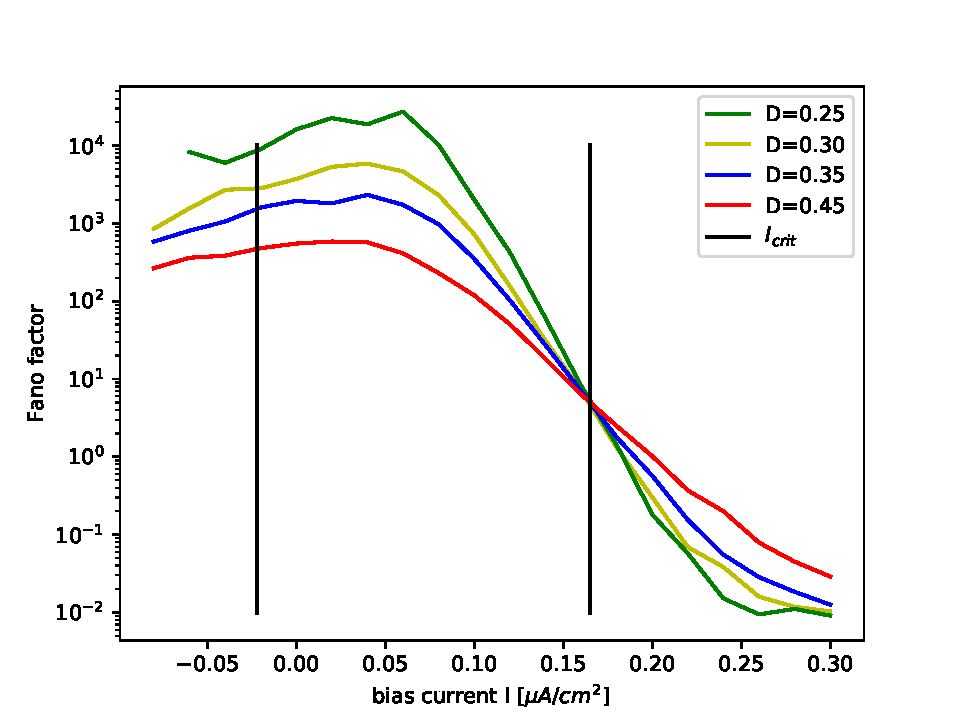
\includegraphics[scale=1]{fanocrit.pdf}\caption{Fano factors for different noise intensities. The vertical lines mark the critical value of $I$ determined from the curves of $D_{eff}$ (Figure \ref{deff})}
	\label{fano}
\end{figure}
The mean firing rates start at zero, increase monotonically with the bias current and eventually approach the firing rate of the running state. This comes as no surprise considering that the neurons spend the majority of the time in the resting state at low bias currents and most of the time in the running state when $I$ is high. All curves intersect at about $I=0.08$, which roughly corresponds to the maxima of $D_{eff}$. This makes sense as the point where the system will be in either state with equal probabilities will also be the point where diffusion gets maximal.
\begin{figure}[H]
	\centering
	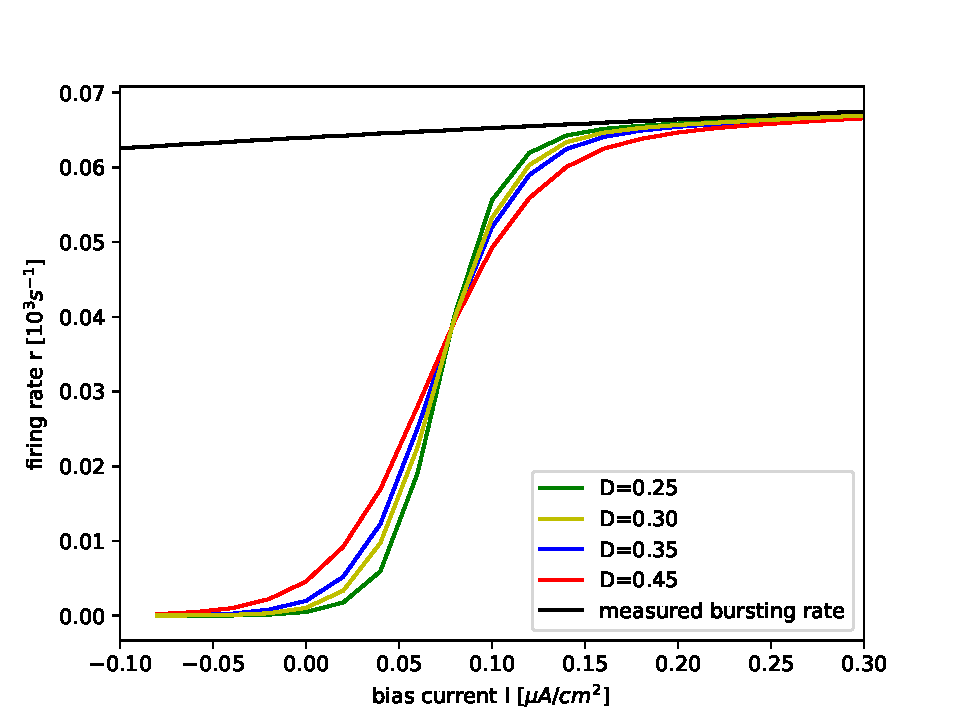
\includegraphics[scale=1]{firingrate.pdf}\caption{Average firing rates for different noise intensities. The black curve denotes the firing rate in the running state which was obtained from a simulation of the system without noise.}
	\label{rate}
\end{figure}
\subsection{Transition rates between the states}
While the spike count may be the most important quantity to determine, there are some other characteristics which should be investigated. An example for these are the transition rates between the states. Looking at the membrane voltage curve over time, both states can be clearly distinguished: in the running state, the voltage oscillates around a value of about -25 $V$, the resting state is characterized by random oscillations with an average voltage of -70 $V$ and the transitions only take a couple tens of microseconds. However, at a given point in time during the simulation, there is no information available about the next time steps. Even more important is the fact that the transition from one state into another is not entirely deterministic but underlies noise. Therefore, a system near the threshold will theoretically undergo infinite transitions before ending up in one of the two states. That is why simply defining a voltage threshold which needs to be crossed does not guarantee correct results for the transition rates. Consequently, another criterion needed to be found. Going back to the condition for counting a spike, a similar criterion can be found for the resting state. Once the system has crossed the resting equilibrium values of the voltage and gating variables in any order (and without firing a spike in between), it is considered to be in the resting state. That way, the current state of the system could be identified much more stable in comparison to a mere voltage threshold.
\subsubsection{Distribution of the state lifetimes}
Now that criteria for transitions between the states have been found, it is possible to investigate the statistics of the running and resting time intervals. In the case of a high number of transitions, the equilibrium as well as the resting time intervals display a simple exponential distribution, indicating that the transitions are random and independent:
\begin{figure}[H]
	\hspace*{-0.5cm}
	\subfigure[]{	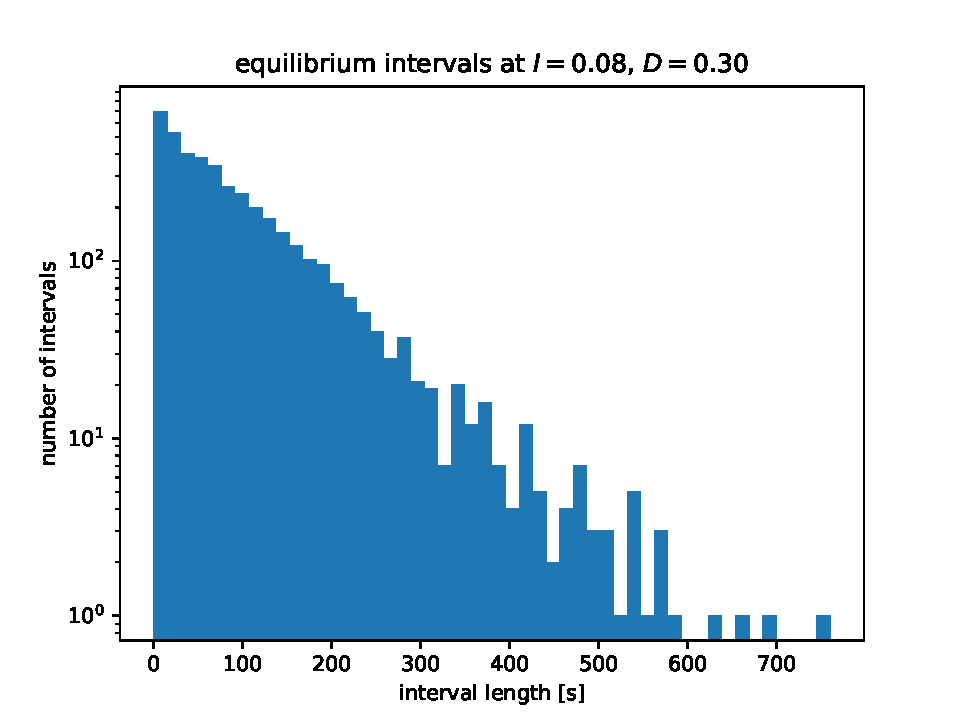
\includegraphics[scale=0.5]{eqdistajrj2newrealfast11jjem2309.pdf}}
	\subfigure[]{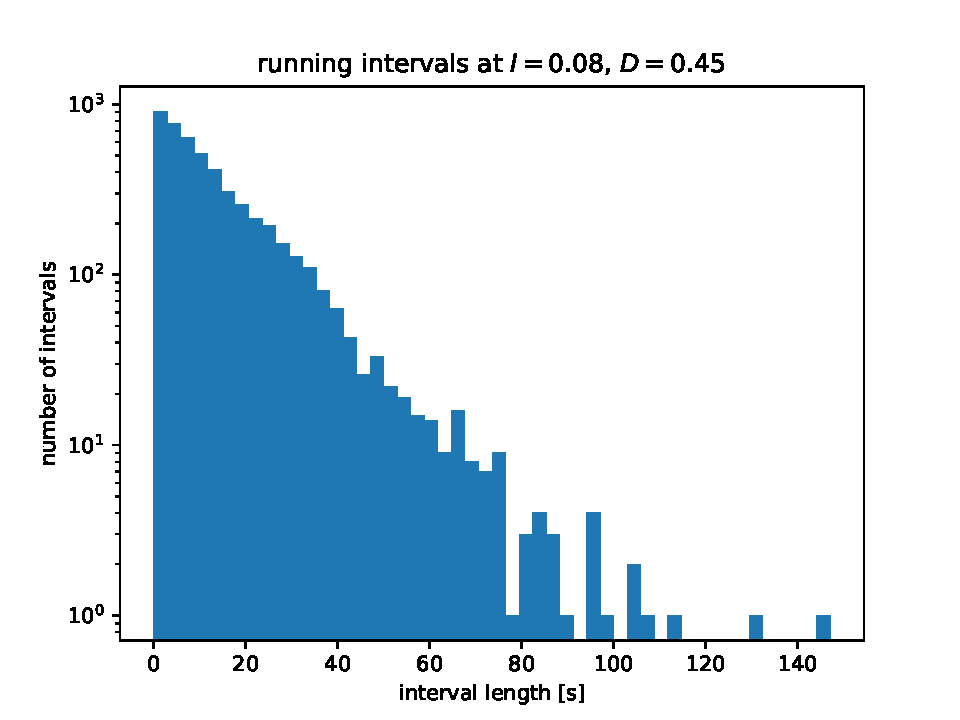
\includegraphics[scale=0.5]{bdistajrj2newrealfast19jjem2st459f.pdf}}
	\caption{Distribution of equilibrium time intervals (left) and running time intervals at high switching rates}
	\label{intdistgood}
\end{figure}
Depending on the noise intensity, the interval lengths can range from some seconds to a few minutes. As the number of events decreases with the interval length, the tail of the distribution gets less regular. Consequently, in the case of a small number of transitions, the whole distribution looks like the tails of the shown histograms.\\
Due to the exponential (and thereby fast decaying) distribution of the intervals, one can now reasonably calculate transition rates.
\begin{figure}[H]
	\centering
	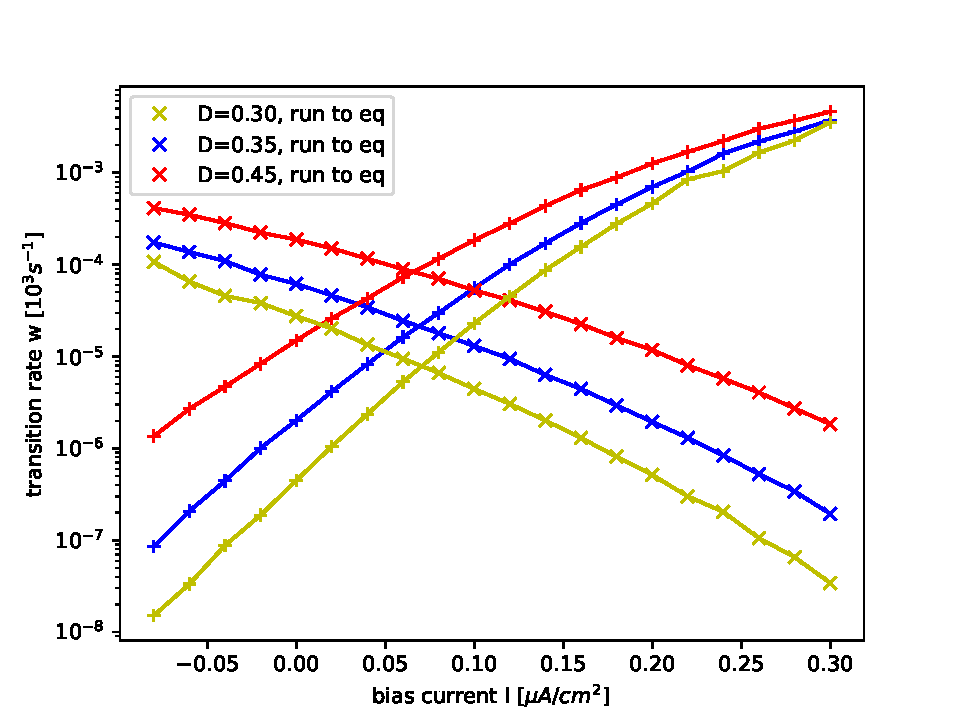
\includegraphics[scale=1]{tranratesneur2.pdf}\caption{Transition rates between the states for a couple different noise intensities}
	\label{tranrateneur}
\end{figure}
As expected, the transition rates grow with the noise intensity. Furthermore, the transition rates from running state to equilibrium decrease with the bias current, while the rates of the opposite transition grow. What this basically means is that the higher the bias current, the higher the likelihood of getting into the running state and the longer are the residence times in this state, which is consistent with the phenomenology of the system. The last observation to discuss here are the intersection points of the rates at the same noise intensity. These can all be found at a bias current of about 0.07 $\mu A/cm^2$, corresponding to the maxima of the effective diffusion coefficients in figure \ref{deff}.
\\
For a given bias current, the transition rates can be put into an Arrhenius plot.
\begin{figure}[H]
	\hspace*{-0.5cm}
	\subfigure[]{	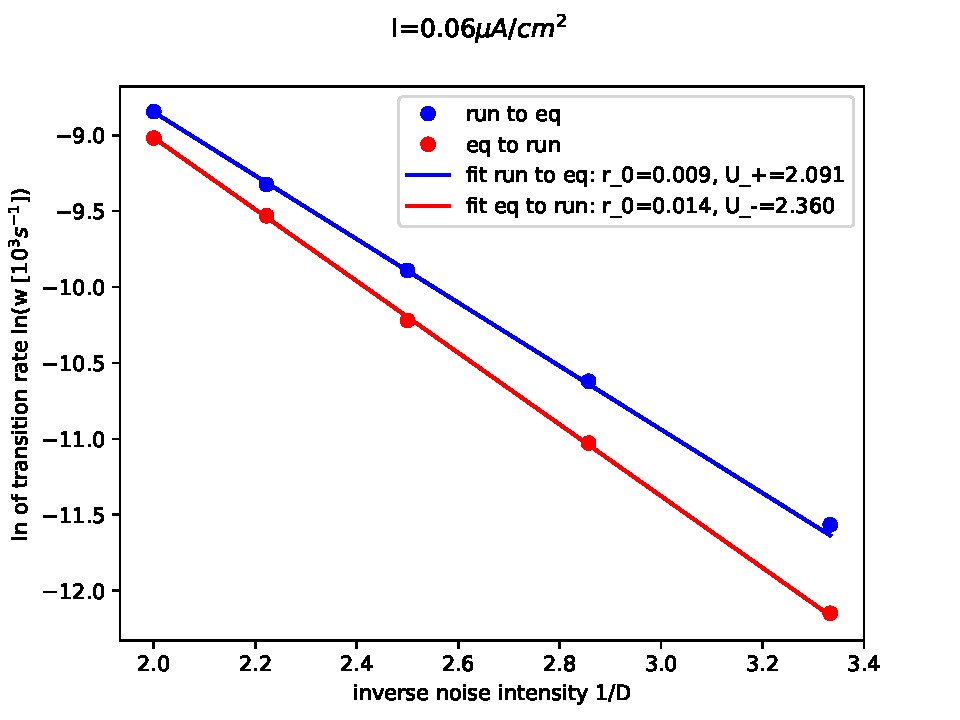
\includegraphics[scale=0.5]{arrheniustotnewrealfast11jjem2shnewrealfast19jjem2stfit7fln.pdf}}
	\subfigure[]{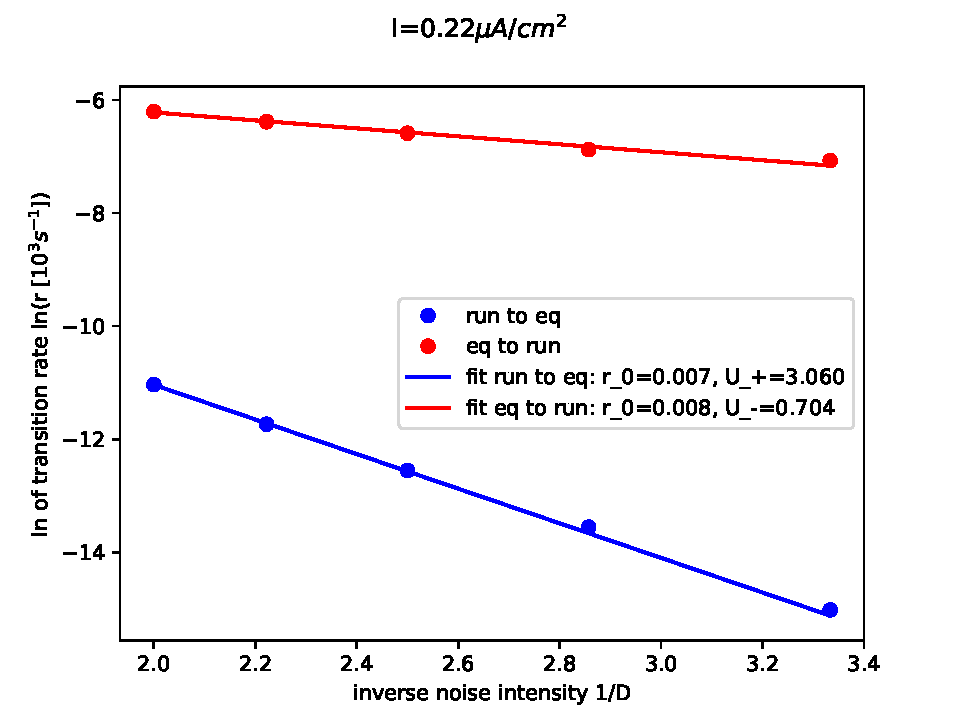
\includegraphics[scale=0.5]{arrheniustotnewrealfast11jjem2shnewrealfast19jjem2stfit15fln.pdf}}
	\caption{logarithm of the transition rates in the middle of the area with giant diffusion (a) and outside of it (b)}
	\label{arrhplots}
\end{figure}
The logarithmic plots illustrate the exponential dependence of the transition rates on the noise intensity at any given bias current. In order to extract effective potential barriers, these data were fit with functions of the form
\begin{align*}
r_{\pm}=r_{0,\pm}\exp\left(-\frac{\Delta U_{\pm}}{D}\right)
\end{align*}
as introduced in section \ref{tst}. 
\bibliography{quellen}
\bibliographystyle{ieeetr}
\section*{Selbst\"andigkeitserkl\"arung}


Ich erkl\"are hiermit, dass ich die vorliegende Arbeit selbst\"andig verfasst und 
noch nicht f\"ur andere Pr\"ufungen eingereicht habe. S\"amtliche Quellen 
einschlie\ss lich Internetquellen, die unver\"andert oder abgewandelt wiedergegeben 
werden, insbesondere Quellen f\"ur Texte, Grafiken, Tabellen und Bilder, sind als 
solche kenntlich gemacht. Mir ist bekannt, dass bei Verst\"o\ss en gegen diese 
Grunds\"atze ein Verfahren wegen T\"auschungsversuchs bzw. T\"auschung eingeleitet 
wird.\\[3cm]
%
\includegraphics{unterschrift_richard}\\ 
Berlin, \dcdatesubmitted
\end{document}

